\section{Hybride Modelle zur Fake News Erkennung}
\label{sec:hybride_modelle}

Hybride Modelle kombinieren die Stärken verschiedener Machine- und Deep-Learning-Ansätze, um die Erkennungsgenauigkeit bei Fake News weiter 
zu verbessern und sowohl semantische als auch stilistische Merkmale effektiv auszuwerten.  
Im Folgenden werden verschiedene hybride Ansätze zur Fake News Erkennung vorgestellt.

\addtocontents{toc}{\protect\setcounter{tocdepth}{1}}

\subsection{CNN und LSTM mit PCA}

In \cite{umer2020} wird eine hybride neuronale Netzwerkarchitektur vorgeschlagen, die die Fähigkeiten von CNN und 
LSTM kombiniert. Dabei kommen zwei unterschiedliche Verfahren zur Dimensionsreduktion zum Einsatz: 
Hauptkomponentenanalyse (PCA) und Chi-Quadrat-Verfahren. 
Diese Verfahren werden empfohlen, um die Dimensionalität der 
Merkmalsvektoren zu verringern, bevor diese an den Klassifikator weitergeleitet werden.

\begin{figure}[htbp]
    \begin{center}
    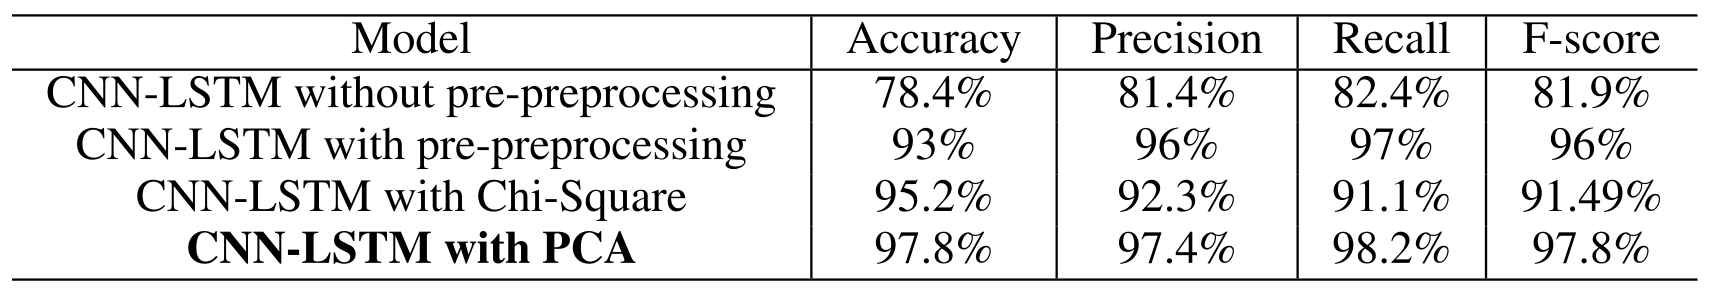
\includegraphics[scale=0.4]{static/cnn_lstm_pca.png}
    \caption{\label{fig:cnn_lstm_pca} Ergebnisse der Klassifizierungen der verschiedenen CNN-LSTM Modelle \cite{umer2020}}
    \end{center}
\end{figure}

Wie in Abbildung \ref{fig:cnn_lstm_pca} zu erkennen, werden verschiedenen Modelle miteinander verglichen. Einmal mit und ohne Vorverarbeitung
der Daten und dann mit den verschiedenen Dimensionsreduktionen PCA und Chi-Quadrat.
PCA schneidet mit einem F1-Score von 97,8\% am Besten ab, während keine Vorverarbeitung der Daten nur einen F1-Score von 81,9\% erreicht.

Die Modelle wurden auf Basis des FNC-1 Datensatzes gemessen, in welchem 2.587 Artikeln etwa 300 verschiedenen Schlagzeilen zugeordnet werden sollen.
Jeder Artikel wird in Bezug auf eine Schlagzeile einer von vier Klassen zugeordnet:

\begin{itemize}
    \item \textbf{Agree:} Artikel stimmt der Schlagzeile zu
    \item \textbf{Disagree:} Artikel widerspricht der Schlagzeile
    \item \textbf{Discuss:} Artikel diskutiert das Thema der Schlagzeile
    \item \textbf{Unrelated:} Artikel ist thematisch nicht verwandt mit der Schlagzeile
\end{itemize}

Zum Vergleich wurden weitere Modelle wie BERT auf den Datensatz angewendet.
Dieses erzielte eine Accuracy von 91,3\% während das hybride CNN-LSTM Modell eine Accuracy von 97,8\% erreichte.

\subsection{CNN und LSTM mit GloVe}

Ein weiteres in \cite{Buddhadev2025} vorgestelltes hybrides Modell ist zusammengesetzt aus CNN und LSTM. Zusätzlich werden die Daten
mit dem GloVe Embedding vorverarbeitet.

\begin{figure}[htbp]
    \begin{center}
    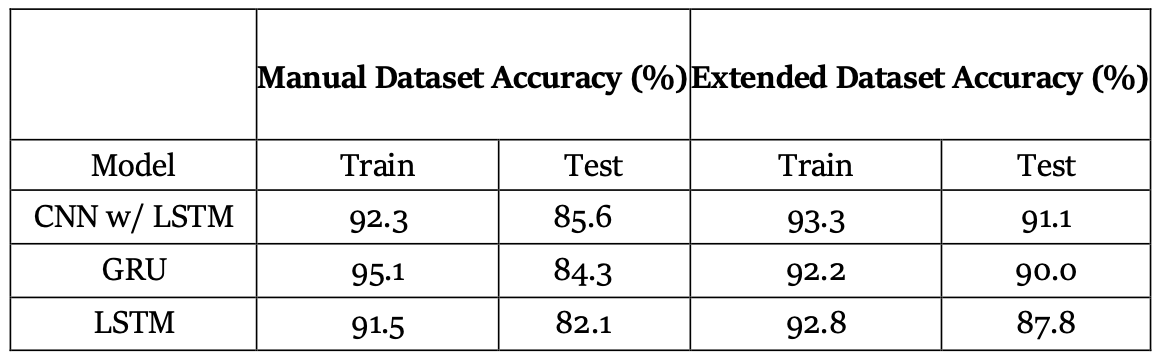
\includegraphics[scale=0.5]{static/cnn_lstm_glove.png}
    \caption{\label{fig:cnn_lstm_glove} Ergebnisse verschiedener Modelle mit GloVe Embedding \cite{Buddhadev2025}}
    \end{center}
\end{figure}

Getestet wurden die Modelle CNN mit LSTM, GRU und LSTM. Genutzt wurden zwei verschiedene Datensätze. Ein manuell erzeugter aus über 1500 Quellen basierend auf
ca. 9000 Artikeln mit Falschinhalten und ca. 9000 echten Artikeln und ein erweiteter, welcher zusätzlich mit Inhalten aus anderen Datensätzen von Kaggle oder
GitHub bereichert wurde.
Durch die zusätzliche Nutzung von GloVe Embeddings wird in dieser Arbeit das Overfitting reduziert (siehe Abbildung \ref{fig:cnn_lstm_glove}).
Vergleichsweise ist die Accuracy beim erweiterten Datensätz mit dem Keras Embedding bei 98,4\% im Training und bei 89,5\% beim Test (CNN mit LSTM).

\cite{Buddhadev2025} stellt außerdem fest, dass Wort-Embeddings wie GloVe die Semantik des Textes deutlich besser erfassen als Techniken zur Merkmalsextraktion 
wie Bag-of-Words oder TF-IDF. In Kombination mit Deep-Learning-Modellen liefern sie eine höhere Genauigkeit als herkömmliche Machine-Learning-Modelle.

\subsection{BERT und CNN (FakeBERT)}
\label{sec:fakebert}

Ein von \cite{Kaliyar:2021aa} vorgestelltes Modell trägt den Namen \textit{FakeBERT} und setzt sich aus den Modellen BERT und CNN zusammen.
BERT analysiert den Text und versteht den 
Zusammenhang der Wörter, während mehrere kleine CNNs gleichzeitig verschiedene Merkmale aus dem Text herausfiltern. Die Ergebnisse dieser 
CNNs werden zusammengeführt, weiterverarbeitet und klassifiziert. Entschieden wird auch in diesem Modell ob es sich um echte oder falsche 
Nachrichten handelt. Das Modell erkennt durch diese Architektur sowohl den allgemeinen Sinn als auch feine sprachliche Muster im Text.

Gearbeitet wurde mit dem \textit{fake-and-real-news-dataset} von Kaggle. Dieser besteht aus 20.800 Nachrichtenartikeln, die während der US-Präsidentschaftswahl 2016 gesammelt wurden. 
Enthalten sind unter anderem Merkmale wie Titel, Autor, Textinhalt. Klassifiziert werden die Nachrichten als echt oder gefälscht. 
Im Datensatz gibt es 10.540 echte und 10.260 gefälschte Artikel.

\begin{figure}[htbp]
    \begin{center}
    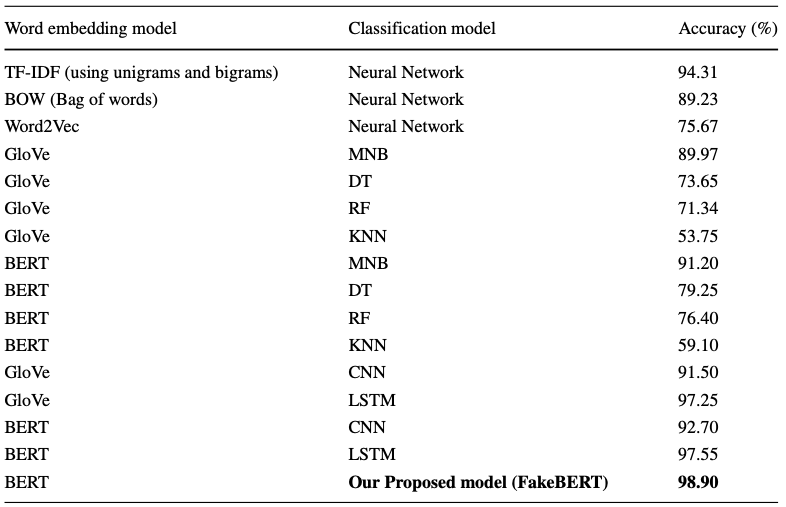
\includegraphics[scale=0.5]{static/bert_cnn_fakebert.png}
    \caption{\label{fig:bert_cnn_fakebert} Ergebnisse der verschiedenen Modelle bei Validierung \cite{Kaliyar:2021aa}}
    \end{center}
\end{figure}

\cite{Kaliyar:2021aa} zeigt, dass das vorgeschlagene Modell FakeBERT mit einer Genauigkeit von 98,90\% (siehe Abbildung \ref{fig:bert_cnn_fakebert})
deutlich besser abschneidet als klassische Machine-Learning-Modelle und bis 2021 bestehende Deep-Learning-Ansätze. Durch die Kombination von BERT als 
kontextuelles Sprachmodell mit mehreren parallel laufenden CNN-Blöcken zur Merkmalsextraktion können sowohl globale Bedeutungszusammenhänge als auch 
lokale sprachliche Muster zuverlässig erfasst werden.

\subsection{BERT und CNN (MCred)}

Wie auch in Kapitel \ref{sec:fakebert} entwickelt \cite{Verma:2023aa} in seiner Arbeit ein weiteres hybrides Modell aus BERT und CNN.
Dieses trägt den Namen \textit{MCred}.

Es wurde auf vier verschiedenen Datensätzen trainiert:
\begin{itemize}
  \item \textbf{WELFake:} Enthält 37.106 gefälschte und 35.028 echte Nachrichten und dient als Hauptdatensatz für das MCred-Modell.
  \item \textbf{Kaggle Fake News Dataset:} Umfasst 10.369 gefälschten und 10.349 echte Nachrichten mit den Merkmalen Titel, Text und Autor. 
  \item \textbf{McIntire Dataset:} Besteht aus 3.164 gefälschten und 3.171 echten Nachrichtenartikeln zur US-Präsidentschaftswahl 2016.
  \item \textbf{FakeNewsNet:} Enthält 24.396 gefälschte und 13.614 echte Nachrichten. Stammt aus diversen Quellen und deckt zahlreiche Themenfelder ab.
\end{itemize}

FakeBERT kombiniert BERT direkt mit parallelen CNNs zur Merkmalsextraktion, während MCred BERT und CNN getrennt verarbeitet und 
ihre Ausgaben später zusammenführt. Zudem nutzt MCred zusätzlich GloVe-Embeddings, was FakeBERT nicht tut. 
Wie in Abbildung \ref{fig:bert_cnn_mcred} zu erkennen erreicht MCred dadurch im Kaggle Datensatz mit einer Accuracy von 99,46\% 
einen besseren Wert als FakeBERT (Rohit Kumar Kaliyar and Narang (2021)) mit 98,90\%.

\begin{figure}[htbp]
    \begin{center}
    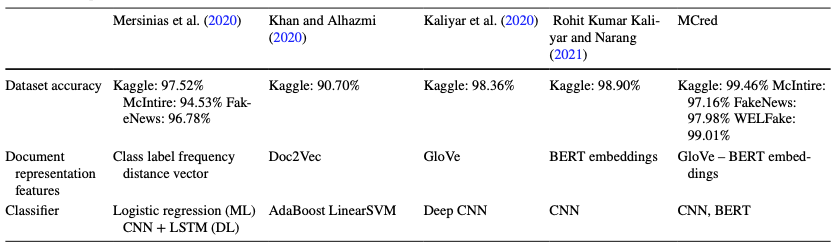
\includegraphics[width=\linewidth]{static/bert_cnn_mcred.png}
    \caption{\label{fig:bert_cnn_mcred} Ergebnisse der verschiedenen Modelle \cite{Verma:2023aa}}
    \end{center}
\end{figure}

In \cite{Dhiman:2024aa} wurde MCred im August 2024 mit einer Accuracy von 99,01\% als zweitbeste State-of-the-Art-Technik benannt.

\subsection{BERT und LSTM}

\cite{RAI202298} schlägt ein hybrides Modell vor, welches BERT und LSTM kombiniert. Hierbei fungiert BERT nachdem die Daten bereinigt wurden als Tokenizer und
Basismodell durch seine Fähigkeit zur tiefen und kontextuellen Wortrepräsentationen (siehe Abbildung \ref{fig:bert_lstm_architecture}). 
Anschließend werden die erzeugten Embeddings in ein LSTM gegeben, in welchem dessen Zellen die Langzeitabhängigkeiten aus den Sequenzen speichern.

\begin{figure}[htbp]
    \begin{center}
    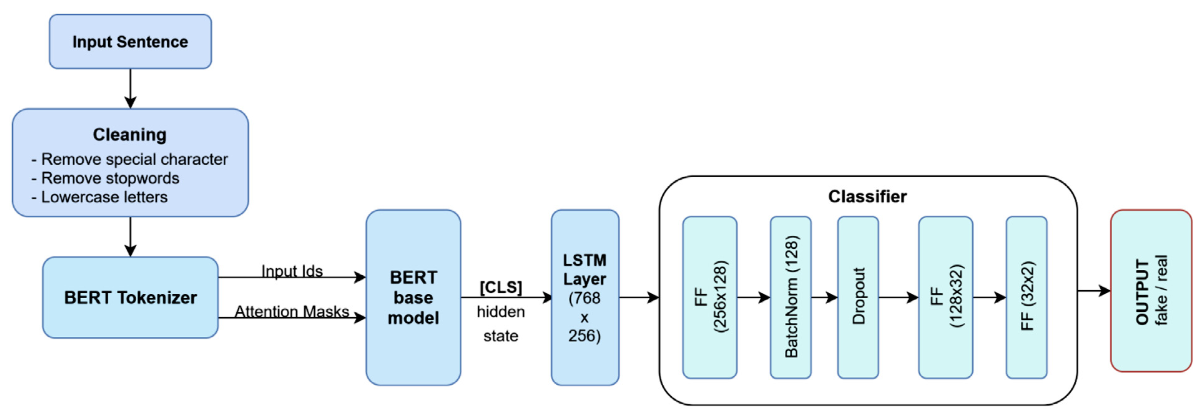
\includegraphics[width=\linewidth]{static/bert_lstm_architecture.png}
    \caption{\label{fig:bert_lstm_architecture} Architekture des vorgeschlagenen hybriden Modells  \cite{RAI202298}}
    \end{center}
\end{figure}

Ziel des Papers ist es, die semantische Tiefe von BERT mit der temporalen Lernfähigkeit von LSTM zu verbinden, um Fake-News besser erkennen zu können.

Für die Evaluation wurde der FakeNewsNet-Datensatz verwendet. Dieser besteht aus dem PolitiFact- und dem GossipCop-Datensatz. 
PolitiFact enthält politisch orientierte Nachrichten, während GossipCop Nachrichten aus dem Unterhaltungsbereich beinhaltet. 
In beiden Datensätzen sind die Inhalte kategorisiert in echte und gefälschte Nachrichten. 
Die Datensätze bestehen aus Nachrichtentiteln. PolitiFact umfasst 432 falsche und 624 echte Titel, GossipCop 5323 falsche und 16.817 echte Titel.

\begin{figure}[htbp]
    \begin{center}
    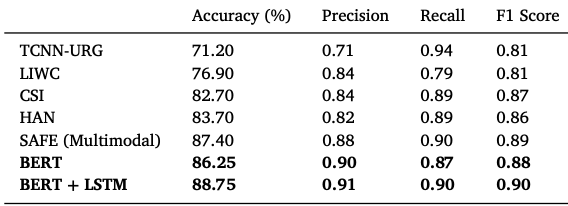
\includegraphics[scale=0.5]{static/bert_lstm_politifact.png}
    \caption{\label{fig:bert_lstm_politifact} Ergebnisse der verschiedenen Modelle mit dem PolitiFact Datensatz \cite{RAI202298}}
    \end{center}
\end{figure}

Das vorgeschlagene Modell, übertrifft klassische Methoden und auch reines BERT in der Fake-News-Erkennung. 
Auf dem PolitiFact-Datensatz erreicht es 88,75\% Genauigkeit (siehe Abbildung \ref{fig:bert_lstm_politifact}, bei reinem BERT sind es nur 86,25\%.
Der LSTM-Layer verbessert dabei die Nutzung der kontextuellen BERT-Embeddings, insbesondere bei der Analyse sprachlicher Muster in Newstiteln.

\subsection{BERT und BiLSTM}

\cite{wang2021covid19fakenewsdetection} stellt ein hybrides BERT und BiLSTM Modell vor. Hierbei wird ein vortrainiertes BERT-Modell als 
Merkmalsencoder genutzt. Dabei bleiben alle internen Gewichte und Parameter von BERT unverändert und werden nicht weiter trainiert. 
Zusätzlich wird ein BiLSTM Modell für die weitere Verarbeitung der BERT-Ausgaben trainiert (siehe Abbildung \ref{fig:bert_bilstm_architecture}).

Verwendet wurde ein COVID-19 Fake News Dataset von Kaggle, bestehend aus 6.420 Trainings- und 2.140 Testeinträgen. 
Jeder Eintrag enthält die Merkmale Tweet-ID, den Text des Tweets und ein Label (echt oder gefälscht).
Mit etwa 8.500 Einträge ist der COVID-19-Datensatz zu klein, um das BERT-Modell effektiv und ohne Overfitting neu zu trainieren.
Bei einem weiteren Training mit diesem Datensatz besteht die Gefahr, dass die vortrainierten Sprachmuster überschrieben werden. 
Die allgemeine Sprachkompetenz von BERT bleibt erhalten, während das darauf aufbauende BiLSTM lernt, 
diese Informationen für die Fake-News-Erkennung zu nutzen.

Verglichen wurde von \cite{wang2021covid19fakenewsdetection} folgende Modelle:
\begin{itemize}
    \item \textbf{Modell 1:} Feinjustiertes BERT-Modell (ohne zusätzliche Schichten)
    \item \textbf{Modell 2:} BERT mit eingefrorenen Parametern + CNN-Schichten
    \item \textbf{Modell 3:} BERT mit nicht eingefrorenen Parametern + CNN-Schichten
    \item \textbf{Modell 4:} BERT mit eingefrorenen Parametern + BiLSTM-Schichten
    \item \textbf{Modell 5:} BERT mit nicht eingefrorenen Parametern + BiLSTM-Schichten
\end{itemize}

\begin{figure}[htbp]
    \begin{center}
    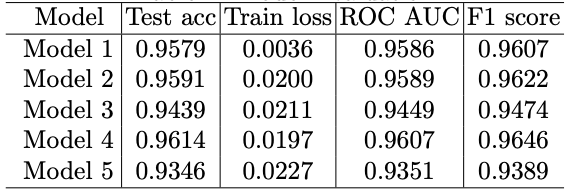
\includegraphics[scale=0.4]{static/bert_bilstm_results.png}
    \caption{\label{fig:bert_bilstm_results} Ergebnisse der verschiedenen Modelle \cite{wang2021covid19fakenewsdetection}}
    \end{center}
\end{figure}

Wie in Abbildung \ref{fig:bert_bilstm_results} zu sehen, hat das Modell 4 mit einer Test Accuracy von 96,14\% und einem F1-Score von 96,46\%
das beste Ergebnis.
Die Kombination aus dem beiden BERT und BiLSTM-Schichten liefert folglich den besten Ansatz zur COVID-19-Fake-News-Erkennung. 
Die Ergebnisse zeigen, dass sich die semantische Tiefe von BERT und sequentielle Kontextverarbeitung von BiLSTM gut ergänzen.

\subsection{BERT und LightGBM}
\label{sec:bert_lightgbm}

\cite{Essa:2023aa} entwickelte ein weiteres hybrides Modell welches das BERT-Embedding und ein LightGBM Modell nutzt.
Das Modell kombiniert die tiefen semantischen Sprachmerkmale von BERT mit der schnellen, skalierbaren Klassifikationsfähigkeit von LightGBM.
Im vorgestellten hybriden Modell wird die Eingabe mittels BERT verarbeitet (siehe Abbildung \ref{fig:bert_lightgbt_architecture}). 
Dabei wird der [CLS]-Token aus den letzten drei Encoderschichten extrahiert und zu einem einzigen Merkmalsvektor zusammengeführt. 
Dieser Vektor dient als Eingabe für LightGBM, das eine binäre Klassifikation in „wahr“ oder „falsch“ vornimmt.

\begin{figure}[htbp]
    \begin{center}
    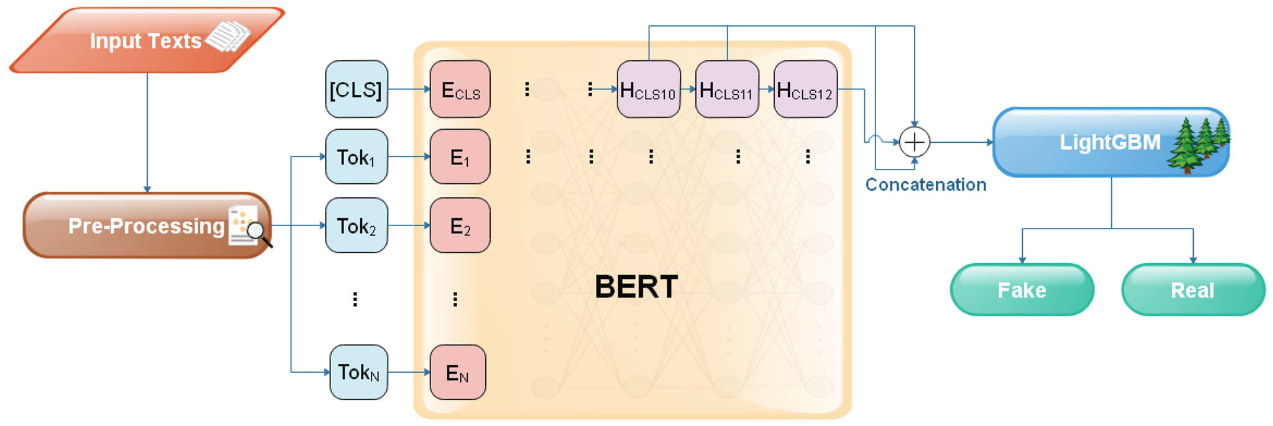
\includegraphics[scale=0.32]{static/bert_lightgbt_architecture.png}
    \caption{\label{fig:bert_lightgbt_architecture} Architektur des hybriden Modells \cite{Essa:2023aa}}
    \end{center}
\end{figure}

Genutzt werden in dem Paper folgende drei Datensätze:
\begin{itemize}
  \item \textbf{ISOT}: Enthält ca. 45.000 Artikel, gleichmäßig auf echte und gefälschte Nachrichten verteilt. 
  Die echten Artikel stammen von Reuters, die gefälschten von fragwürdigen Quellen laut PolitiFact. 
  Themenschwerpunkte sind Politik und Weltgeschehen (2016–2017).

  \item \textbf{TI-CNN}: Besteht aus 20.015 Artikeln (8074 echt, 11.941 falsch). Die echten Nachrichten stammen von renommierten Medien 
  wie der New York Times, die gefälschten von über 240 inoffiziellen Webseiten.

  \item \textbf{FNC (Fake News Corpus)}: Umfasst Millionen Artikel von über 1000 Domains. Für die Experimente wurde ein ausgeglichener 
  Datensatz aus je 500.000 echten und gefälschten Artikeln erstellt. Enthält zusätzliche Metadaten wie Titel, Autor und URL.
\end{itemize}

\begin{figure}[htbp]
    \begin{center}
    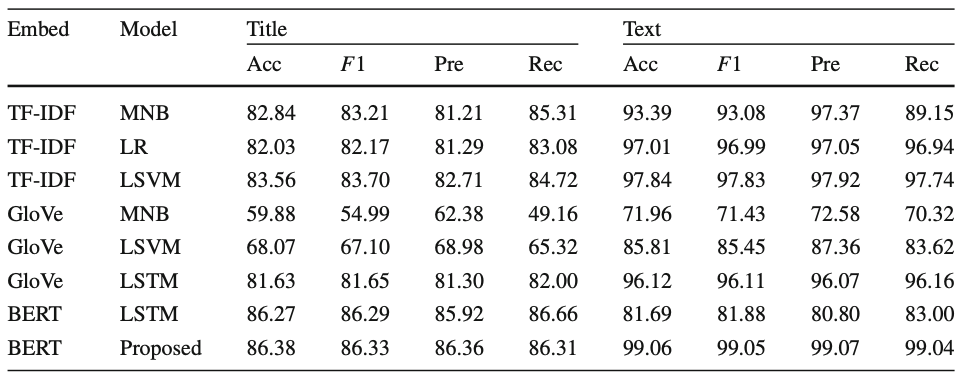
\includegraphics[scale=0.4]{static/bert_lightgbt_results.png}
    \caption{\label{fig:bert_lightgbt_results} Ergebnisse der verschiedenen Modelle auf dem FNC-Datensatz \cite{Essa:2023aa}}
    \end{center}
\end{figure}

In Abbildung \ref{fig:bert_lightgbt_results} zu sehen ist, dass dieses Modell anderen gerade bei großen Datenmengen überlegen ist.
\cite{Dhiman:2024aa} nennt dieses Modell im August 2024 mit einer Accuracy von 99,06\% die beste State-of-the-Art-Technik.


\subsection{RoBERTa und LightGBM}
\label{sec:roberta_lightgbm}

Aufbauend auf dem hybriden BERT und LightGBM Model zeigt \cite{V_G_2024} die Vorteile eines hybriden RoBERTa-LightGBM Modells.

RoBERTa ist eine weiterentwickelte und leistungsstärkere Version von BERT, die durch effizienteres Training und größere Datenbasis 
bessere Ergebnisse in der Fake-News-Erkennung erzielt. 
Statt mit den 16GB Textdaten des BERT Modells wurde RoBERTa mit über 160GB trainiert, wodurch eine deutlich bessere Generalisierungsfähigkeit besteht.
Durch RoBERTAs fortgeschritteneres dynamisches Maskieren wird jedes mal genau dann ein Maskierungspattern generiert, wenn eine Sequenz einem Modell hinzugefügt wird \cite{roberta:main}.

Das Paper verwendet den „Fake News Detection Dataset“ zum Training. 
Die Daten stammen von reuters.com und umfassen jeweils 12.600 Artikel, gesammelt in den Jahren 2016 bis 2017.

Nach der Vorverarbeitung wurden die Daten tokenisiert und mit Roberta in Vektor-Embeddings umgewandelt.
Verwendet wird der [CLS] Token aus den letzten drei Hidden Layers, um den gesamten Text zu repräsentieren.
Durch Self Attention liefert dies eine feste, dichte Vektor-Repräsentation pro Artikel.
Diese Embeddings dienten anschließend als Eingabe für LightGBM zur binären Klassifikation.

RoBERTa-LightGBM erzielt eine Verbesserung gegenüber BERT-LightGBM von bis zu 21\% (siehe Abbildung \ref{fig:roberta_lightgbm_auc_roc_value}).

\begin{figure}[htbp]
    \begin{center}
    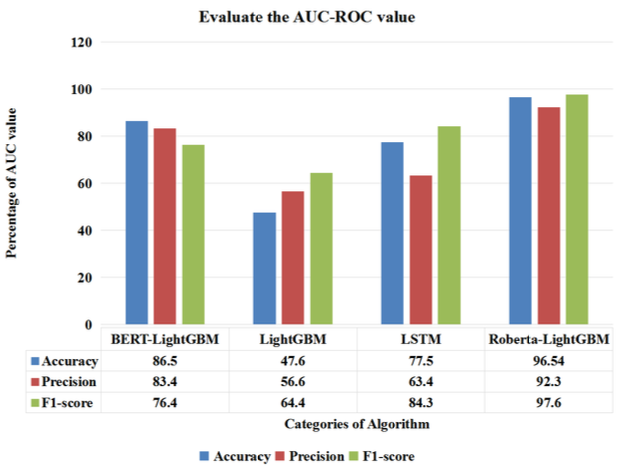
\includegraphics[scale=0.5]{static/roberta_lightgbm_auc_roc_value.png}
    \caption{\label{fig:roberta_lightgbm_auc_roc_value} Vergleich der Ergebnisse der verschiedenen Modelle \cite{V_G_2024}}
    \end{center}
\end{figure}

\addtocontents{toc}{\protect\setcounter{tocdepth}{2}}